\chapter{Algebra}\label{chapter:algebra}

    For the later sections on (co)homology theory, some terminology from \cref{chapter:hom_alg} is used. Basic introductions to group theory can be found in~\citet{jeevanjee_introduction_2015,wigner_group_2012}.

    \minitoc

\section{Algebraic structures}

    \newdef{Semigroup}{\index{semi-!group}\index{magma}\label{algebra:semigroup}
        A set $G$ equipped with a binary operation $\star$ such that the following axioms are satisfied:
        \begin{enumerate}
            \item\textbf{Closure}: $G$ is closed under $\star$.
            \item\textbf{Associativity}: $\star$ is associative.
        \end{enumerate}
        If the associativity axiom is dropped, a \textbf{magma} is obtained.
    }

    \newdef{Monoid}{\index{monoid}\label{algebra:monoid}
        A set $M$ equipped with a binary operation $\star$ such that the following axioms are satisfied:
        \begin{enumerate}
            \item\textbf{Closure}: $M$ is closed under $\star$.
            \item\textbf{Associativity}: $\star$ is associative.
            \item\textbf{Unitality}: $M$ has an identity element $e$ with respect to $\star$.
        \end{enumerate}
    }
    \newdef{Nilpotent}{\index{nilpotent}\label{algebra:nilpotent}
        An element $x$ of a monoid $(M,\star,e)$ for which there exists an integer $k\in\mathbb{N}$ such that $x^k=e$, where $x^k:=\underbrace{x\star\cdots\star x}_{k\text{ times}}$.
    }
    \begin{property}[Eckmann--Hilton argument]\index{Eckmann--Hilton!argument}\index{commutativity}\index{Abel|seealso{commutativity}}\label{algebra:eckmann_hilton}
        Let $(M,\circ),(M,\otimes)$ be two monoid structures (or even unital magma structures) on the same set $M$ such that
        \begin{gather}
            (a\circ b)\otimes(c\circ d) = (a\otimes c)\circ(b\otimes d)
        \end{gather}
        for all $a,b,c,d\in M$. The two monoid structures coincide and are in fact \textbf{Abelian}, i.e.~they are \textbf{commutative}:
        \begin{gather}
            a\circ b = b\circ a
        \end{gather}
        for all $a,b\in M$.
    \end{property}
    \begin{remark}
        This property admits a vast generalization. See \cref{cat:eckmann_hilton} for more information.
    \end{remark}

    \newdef{Group}{\index{group}
        A set $G$ equipped with a binary operation $\star$ such that the following axioms are satisfied:
        \begin{enumerate}
            \item\textbf{Closure}: $G$ is closed under $\star$.
            \item\textbf{Associativity}: $\star$ is associative.
            \item\textbf{Unitality}: $G$ has an identity element $e$ with respect to $\star$.
            \item\textbf{Inverses}: Every element in $G$ has an inverse with respect to $\star$.
        \end{enumerate}
    }
    \newnot{Identity element}{
        Although the identity element of a group is generally denoted by $e$, in certain cases, whenever this makes sense, the identity element will be denoted by 0 or 1 (additive and multiplicative conventions).
    }

    \newdef{Abelian group}{\index{commutativity}\index{Abelian!group}
        Let $(G,\star)$ be a group. If $\star$ is commutative, then $G$ is said to be an Abelian or \textbf{commutative} group.
    }

    \newdef{Morphism}{\index{morphism!of groups}
        A group \textbf{(homo)morphism} $\Phi:(G,\star,e_G)\rightarrow(H,\cdot,e_H)$ is a function $\Phi:G\rightarrow H$ such that
        \begin{gather}
            \Phi(g\star g') = \Phi(g)\cdot\Phi(g')
        \end{gather}
        for all $g,g'\in G$. Note that this also implies that $\Phi(e_G)=e_H$.
    }

    \newdef{Kernel}{\index{kernel}\label{group:kernel}
        The kernel of a group morphism $\Phi:G\rightarrow H$ is defined as the set
        \begin{gather}
            \ker(\Phi) := \{g\in G\mid\Phi(g)=e_H\}.
        \end{gather}
        This set carries a group structure induced by that on $G$.
    }

    \begin{theorem}[First isomorphism theorem]\index{isomorphism theorem}\label{group:first_isomorphism_theorem}
        Consider a group morphism $\Phi:G\rightarrow H$. If $\Phi$ is surjective, then $G/\ker(\Phi)\cong H$.
    \end{theorem}

\section{Group theory}\label{section:groups}

    \newdef{Order of a group}{\index{order!of a group}
        The number of elements in the group. It is denoted by $|G|$ or $\mathrm{ord}(G)$.
    }
    \newdef{Order of an element}{
        The order of an element $a\in G$ is the smallest integer $n\in\mathbb{N}$ such that
        \begin{gather}
            a^n = e\,,
        \end{gather}
        where $e$ is the identity element of $G$.
    }

    \newdef{Torsion group}{\index{torsion!group}\label{group:torsion_group}
        A group in which all elements have finite order. The torsion set $\mathrm{Tor}(G)$ of a group $G$ is the set of all elements $a\in G$ that have finite order. If $G$ is Abelian, $\mathrm{Tor}(G)$ is a subgroup.
    }

    \begin{theorem}[Lagrange]\index{Lagrange}
        Let $G$ be a finite group and let $H$ be a subgroup. Then $|H|$ is a divisor of $|G|$.
    \end{theorem}
    \begin{result}
        The order of any element $g\in G$ is a divisor of $|G|$.
    \end{result}

    \begin{construct}[Grothendieck completion]\index{Grothendieck!completion}\label{group:grothendieck_completion}
        Let $(A,\oplus)$ be a commutative monoid. From this monoid, one can construct an Abelian group $G(A)$, called the Grothendieck completion of $A$, as the quotient of $A\times A$ by the equivalence relation
        \begin{gather}
            (a_1,a'_1)\sim (a_2,a'_2)\iff\exists c\in A:a_1\oplus a'_2\oplus c = a'_1\oplus a_2\oplus c\,.
        \end{gather}
        The identity element, denoted by 0, is given by the equivalence class of $(0,0)$. By the definition of $G(A)$, this class contains all elements in $\Delta_A$. In particular, $[(a,b)]$ is the additive inverse of $[(b,a)]$:
        \begin{gather}
            [(a,b)] + [(b,a)] = 0\,.
        \end{gather}
    \end{construct}
    \begin{uproperty}
        Let $G(A)$ be the Grothendieck completion of the Abelian monoid $A$. Every monoid morphism $m:A\rightarrow B$ between $A$ and an Abelian group factors uniquely through a group morphism $\varphi:G(A)\rightarrow B$.
    \end{uproperty}

    \begin{example}[Integers]
        The Grothendieck completion of the natural numbers $\mathbb{N}$ is the additive group of integers $\mathbb{Z}$.
    \end{example}

\subsection{Abelian groups}

    \newdef{Commutator subgroup}{\index{commutator!subgroup}\index{derived!subgroup}\index{derived!series}
        The commutator subgroup or \textbf{derived subgroup} $[G,G]$ of $G$ is defined as the group generated by the \textbf{commutators}
        \begin{gather}
            [g,h] := g^{-1}h^{-1}gh\,,
        \end{gather}
        where $g,h\in G$. The \textbf{derived series} of a group $G$ is defined as the following sequence:
        \begin{gather}
            G\subseteq[G,G]\subseteq\bigl[[G,G],[G,G]\bigr]\subseteq\cdots
        \end{gather}
        To ease the notation, these groups are often denoted by $G^{(i)}$: $G^{(0)}:=G$ and $G^{(i)}:=[G^{(i-1)},G^{(i-1)}]$.
    }
    \newdef{Solvable group}{\index{group!solvable}\label{group:solvable}
        A group whose derived series ends in the trivial group.
    }

    \begin{property}[Abelianization]\index{Abelianization}\label{group:abelianization}
        The Abelianization $G/[G,G]$ is an Abelian group. Moreover, a group $G$ is Abelian if and only if $[G,G]$ is trivial.
    \end{property}
    \begin{result}[Abelian quotients]
        A quotient group $G/H$ is Abelian if and only if $[G,G]\leq H$.
    \end{result}

\subsection{Cosets}\index{co-!set}

    \newdef{Coset}{\index{normal!subgroup}\index{invariant!subgroup|see{normal subgroup}}\index{divisor}\label{group:coset}
        Let $G$ be a group and let $H$ be a subgroup. The left coset of $H$ with respect to $g\in G$ is defined as the set
        \begin{gather}
            gH := \{gh\mid h\in H\}\,.
        \end{gather}
        The right coset is defined analogously. If for all $g\in G$, the left and right cosets coincide, the subgroup $H$ is said to be a \textbf{normal subgroup}, \textbf{normal divisor} or \textbf{invariant subgroup}.
    }
    \begin{notation}
        The set of left (resp.~right) cosets is denoted by $G/H$ (resp.~$H\backslash G$).
    \end{notation}

    \newdef{Index}{\index{index!of a subgroup}\label{group:index}
        Let $G$ be a group and let $H$ be a subgroup. The index $|G:H|$ of $H$ in $G$ is defined as the number of cosets $H$ in $G$. This can also be expressed as
        \begin{gather}
            |G| = |G:H||H|\,.
        \end{gather}
    }
    \begin{property}[Tower law]\index{tower law}\label{group:tower_rule_groups}
        Consider the subgroup inclusions $G\subset H\subset I$.
        \begin{gather}
            [I:G]=[I:H][H:G]
        \end{gather}
    \end{property}

    \newadef{Normal subgroup}{\index{normal!subgroup}\index{conjugacy class}\label{group:normal_subgroup}
        Let $G$ be a group and let $H$ be a subgroup. Consider the \textbf{conjugacy classes} $gHg^{-1}$ for all $g\in G$. If all classes coincide with $H$ itself, then $H$ is said to be a normal subgroup.
    }
    \begin{notation}
        If $N$ is a normal subgroup of $G$, this is often denoted by $N\vartriangleleft G$.
    \end{notation}

    \newprop{Quotient group}{\index{quotient!group}\label{group:quotient_group}
        Let $G$ be a group and let $N$ be a normal subgroup. The coset space $G/N$ can be turned into a group by equipping it with the product induced by that on $G$.
    }

    \newdef{Center}{\index{center}\label{group:center}
        The center of a group $G$ is defined as follows:
        \begin{gather}
            Z(G) := \{z\in G\mid\forall g\in G:zg = gz\}\,.
        \end{gather}
        This is a normal subgroup of $G$.
    }
    \newdef{Normalizer}{\index{normalizer}
        The normalizer of a subset $H\subseteq G$ is defined as follows:
        \begin{gather}
            N_G(H) := \{g\in G\mid gHg^{-1}=H\}=\{g\in G\mid[g,H]=H\}\,.
        \end{gather}
    }
    \newdef{Centralizer}{\index{centralizer}\label{group:centralizer}
        The centralizer of a subset $H\subseteq G$ is defined as follows:
        \begin{gather}
            C_G(H) := \{g\in G\mid\forall h\in H:ghg^{-1}=h\}=\{g\in G\mid[g,H]=0\}\,.
        \end{gather}
        This group clearly satisfies $C_G(H)\triangleleft N_G(H)$.
    }

\subsection{Sylow theorems}\index{Sylow}

    \newdef{Sylow $p$-subgroup}{\index{Sylow!subgroup}
        Consider a finite group $G$. For every prime $p$, a Sylow $p$-subgroup of $G$ is defined as a maximal \textbf{$p$-group} in $G$, i.e.~every element has order a power of $p$ and the subgroup is maximal with respect to this property. The set of all Sylow $p$-subgroups of $G$ is denoted by $\mathrm{Syl}_p(G)$.
    }

    \begin{theorem}[Sylow I]
        Consider a finite group $G$. For every prime factor $p$ of $|G|$ with multiplicity $n$, there exists a Sylow $p$-subgroup of order $p^n$.
    \end{theorem}
    \begin{theorem}[Sylow II]
        Consider a finite group $G$ and a prime factor $p$ of $|G|$. All Sylow $p$-subgroups are conjugate and, in particular, isomorphic.
    \end{theorem}
    \begin{theorem}[Sylow III]
        Consider a finite group $G$ and a prime factor $p$ of $|G|$ of multiplicity $n$ such that $|G|=p^nm$ for some $m\in\mathbb{N}$ and write $n_p:=|\mathrm{Syl}_p(G)|$.
        \begin{itemize}
            \item $m=|G:H|$ for every Sylow $p$-subgroup $H$ of $G$.
            \item $n_p\mid m$, i.e.~$n_p$ divides $m$.
            \item $n_p=1\bmod p$.
            \item $n_p=|G:N_G(H)|$ for any Sylow $p$-subgroup $H$ of $G$.
        \end{itemize}
    \end{theorem}

\subsection{Symmetric groups}

    \newdef{Symmetric group}{\index{symmetric!group}\index{degree!of symmetric group}\label{group:permutation_group}
        The symmetric group $S_n$ (on $n$ elements) is defined as the set of all permutations of $\{1,\ldots,n\}$. The integer $n\in\mathbb{N}$ is called the \textbf{degree} of the symmetric group. The symmetric group $\Sym(X)$ on a finite set $X$ is defined similarly (by enumerating the elements)\footnote{Two such choices are related through conjugation by a unique permutation and, hence, the resulting groups are isomorphic.}.

        For infinite sets $X$, the symmetric group $\Sym(X)$ is defined as the group of all bijections from $X$ to itself (where the multiplication is given by function composition).
    }
    \newdef{Automorphism group}{\index{automorphism}\label{algebra:automorphism}
        Consider a set $X$ with some extra structure (see \cref{chapter:cat} for a more formal treatment), e.g.~a monoid structure or group structure. The subset of $\Sym(X)$ consisting of bijections that preserve this structure, the \textbf{automorphisms} of $X$, inherits the group structure of $\Sym(X)$ and is denoted by $\Aut(X)$.
    }

    \begin{theorem}[Cayley]\index{Cayley}
        Every group $G$ is isomorphic to a subgroup of the permutation group $\Sym(G)$.
    \end{theorem}

    \newdef{Cycle}{\index{cycle}
        A $k$-cycle is a permutation of the form $(a_1\ a_2\ \cdots\ a_k)$ sending $a_i$ to $a_{i+1}$ (and $a_k$ to $a_1$). A \textbf{cycle decomposition} of an arbitrary permutation is the decomposition into a product of disjoint cycles.
    }
    \begin{property}[Cycles are cyclic]
        Let $\tau$ be a $k$-cycle. Then $\tau$ is $k$-cyclic (hence the name): $\tau^k = e$.
    \end{property}
    \begin{example}
        Consider the set $\{1,2,3,4,5,6\}$. The permutation $\sigma:x\mapsto(x+2)\bmod6$ can be decomposed as $\sigma = (1\ 3\ 5)(2\ 4\ 6)$.
    \end{example}

    \newdef{Transposition}{\index{transposition}
        A permutation that exchanges two elements but leaves the other ones unchanged.
    }
    \begin{property}[Decomposition]\index{parity}
        Any permutation can be decomposed as a product of transpositions. A permutation is said to be \textbf{even} (resp.~\textbf{odd}) if the number of transpositions in its decomposition is even (resp.~odd). One can prove that the parity of a permutation is well-defined, i.e.~it is independent of the choice of decomposition.
    \end{property}

    \newdef{Alternating group}{\index{group!alternating}
        The alternating group $A_n$ is the subgroup of $S_n$ containing all even permutations.
    }

    \newdef{Shuffle}{\index{shuffle}\label{group:shuffle}
        A permutation $\sigma\in S_n$ is called a $(p,q)$-shuffle (where $p+q=n$) if there exist disjoint increasing sequences $I=\{i_1<\cdots<i_p\}$ and $J=\{j_1<\cdots<j_q\}$ such that
        \begin{gather}
            \sigma(x) =
            \begin{cases}
                k&\cif x=i_k\,,\\
                k+p&\cif x=j_k\,.
            \end{cases}
        \end{gather}
        The name stems from the idea of dividing a deck of cards into two piles and interleaving them. This way the order in each pile is strictly preserved.

        An unshuffle $\tau\in S_n$ is defined as a permuation such that $\tau^{-1}$ is a shuffle, i.e.~there exist disjoint increasing sequences $I=\{i_1<\cdots<i_p\}$ and $J=\{j_1<\cdots<j_q\}$ such
        \begin{gather}
            \tau(k) =
            \begin{cases}
                i_k&\cif k\leq p\,,\\
                j_{k-p}&\cif k>p\,.
            \end{cases}
        \end{gather}
    }

\subsection{Group presentations}

    \newdef{Generator}{\index{generator}
        A set of elements $\{g_i\}_{i\in I}\subset G$ (where $I$ can be infinite) is said to generate $G$ if every element in $G$ can be written as a finite product of the elements $g_i$ and their inverses. These elements are then called generators of $G$.
    }
    \begin{remark}
        If $G$ is finite, the inverses can themselves be expressed as powers, so inverses are only required for infinite groups.
    \end{remark}

    \newdef{Relation}{\index{relation}
        Let $G$ be a group. If the product of a number of elements $g\in G$ is equal to the identity $e$, this product is said to be a relation on $G$.
    }
    \newdef{Complete set of relations}{
        Let $G$ be a group generated by a set of elements $S$ and let $R$ be a set of relations on $S$. If $G$ is uniquely (up to an isomorphism) determined by $S$ and $R$, the set of relations is said to be complete.
    }

    \newdef{Presentation}{\index{presentation}\label{group:presentation}
        Let $G$ be a group with generators $S$ and let $R$ be a complete set of relations. The pair $(S,R)$ is called a presentation of $G$.

        If $R$ is finite, $G$ is said to be \textbf{finitely related}, while if $S$ is finite, $G$ is said to be \textbf{finitely generated}. If both $S$ and $R$ are finite, $G$ is said to be \textbf{finitely presented}.
    }
    \begin{notation}
        The presentation of a group $G$ is often denoted by $\langle S\mid R \rangle$, where $S$ is the set of generators and $R$ the set of relations.
    \end{notation}

    \begin{remark}
        It should be clear that a group can have many different presentations and that it is (very) difficult to tell if two groups are isomorphic by just looking at their presentations.
    \end{remark}

\subsection{Direct products}

    \newdef{Direct product}{\index{direct product!of groups}\index{component}\label{group:direct_product}
        Let $G,H$ be two groups. The direct product $G\times H$ is defined as the set-theoretic Cartesian product $G\times H$ equipped with a group operation defined as
        \begin{gather}
            (g_1,h_1)\cdot(g_2,h_2) = (g_1g_2,h_1h_2)\,,
        \end{gather}
        where the operations on the right-hand side are the group operations in $G$ and $H$. This definition can be generalized to any number of groups, even an infinite number of them if the $n$-tuples are replaced by elements of the infinite Cartesian product.

        If $g\in G_1\times\cdots\times G_n$ can be written as $(g_1,\ldots,g_n)$ for $g_i\in G_i$, the $g_i$ are called the \textbf{components} of $g$.
    }

    \newdef{Weak direct product}{\index{direct sum!of groups}
        Consider the direct product of groups. The subgroup consisting of all elements for which all components, except finitely many of them, are the identity, is called the weak direct product. In the case of Abelian groups, this is often called the \textbf{direct sum}. For a finite number of groups, the direct product and direct sum coincide.
    }
    \begin{notation}
        The direct sum is often denoted by $\oplus$ (in accordance with the notation for \textit{vector spaces} and other algebraic structures that will be introduced further on).
    \end{notation}

    \newdef{Inner semidirect product}{\index{semi-!direct product}\index{split!product}
        Let $G$ be a group, $H\leq G$ a subgroup and $N\vartriangleleft G$ a normal subgroup. $G$ is said to be the inner semidirect product of $H$ and $N$, denoted by $N\rtimes H$, if it satisfies the following equivalent statements:
        \begin{itemize}
            \item $G = NH := \{nh\mid n\in N,h\in H\}$, where $N\cap H = \{e\}$.
            \item For every $g\in G$, there exist a unique $n\in N,h\in H$ such that $g=nh$.
            \item For every $g\in G$, there exist a unique $n\in N,h\in H$ such that $g=hn$.
            \item There exists a group morphism $\rho:G\rightarrow H$ that satisfies $\rho|_H = e$ and $\ker(\rho)=N$.
            \item The composition of the natural embedding $i:H\rightarrow G$ and the projection $\pi:G\rightarrow G/N$ gives an isomorphism between $H$ and $G/N$.
        \end{itemize}
        Whenever $G$ is isomorphic to $N\rtimes H$, it is said to \textbf{split} over $N$.
    }
    \begin{property}[Normal subgroups]
        If both $H$ and $N$ in the above definition are normal, the inner semidirect product coincides with the direct product. If the subgroups $H$ and $N$ have presentations $\langle S_H\mid R_H \rangle$ and $\langle S_N\mid R_N \rangle$, the direct product is given by
        \begin{gather}
            \label{group:direct_product_presentation}
            H\times N = \langle S_H\cup S_N\mid R_H\cup R_N\cup R_C \rangle\,,
        \end{gather}
        where $R_C$ is the set of relations that enforce the commutativity of $H$ and $N$.
    \end{property}

    \newdef{Outer semidirect product}{
        Let $G,H$ be two groups and let $\varphi:H\rightarrow\Aut(G)$ be a group morphism. The outer semidirect product $G\rtimes_\varphi H$ is defined as the set-theoretic Cartesian product $G\times H$ equipped with a binary relation $\cdot$ such that
        \begin{gather}
            (g_1,h_1)\cdot(g_2,h_2) = \bigl(g_1\varphi(h_1)(g_2),h_1h_2\bigr)\,.
        \end{gather}
        The structure $(G\rtimes_\varphi H,\cdot)$ forms a group.

        By noting that the set $N=\{(g,e_H)\mid g\in G\}$ is a normal subgroup isomorphic to $G$ and that the set $B=\{(e_G,h)\mid h\in H\}$ is a subgroup isomorphic to $H$, one can also construct the outer semidirect product $G\rtimes_\varphi H$ as the inner semidirect product $N\rtimes B$.
    }

    \begin{remark}[Direct products]
        The direct product of groups is a special case of the outer semidirect product where the group morphism is given by the trivial map $\varphi:h\mapsto e_G$.
    \end{remark}

    Semidirect products can even be generalized further.
    \newdef{Bicrossed product of groups\footnotemark}{\index{bicrossed product}\index{matched pair}\index{Zappa--Sz\'ep product}\label{group:bicrossed_product}
        \footnotetext{Also called the \textbf{Zappa--Sz\'ep product}.}
        Consider a group $G$ with two subgroups $K,H\leq G$, with $K\cap H=\{e\}$, such that every element $g\in G$ can be uniquely decomposed as the product of an element in $H$ and an element in $K$. This implies that for $k\in $ and $h\in H$, there exists a unique decomposition of $kh$ of the form
        \begin{gather}
            kh = (k\cdot h)k^h\,,
        \end{gather}
        where $k\cdot h\in H$ and $k^h\in K$.

        It can be checked that the associativity of the product implies that $-\cdot-:K\times H\rightarrow H$ defines a \textit{left action} of $K$ on $H$ and that $-^-:K\times H\rightarrow K$ defines a \textit{right action} of $H$ on $K$ (see \cref{section:group_actions} further on). Some other properties are obtained in the same way:
        \begin{itemize}
            \item $e^h = e$,
            \item $k\cdot e = e$,
            \item $(kk')^h = k^{k'\cdot h}k'^h$, and
            \item $k\cdot(hh') = (k\cdot h)(k^h\cdot h')$.
        \end{itemize}
        Any two groups having this structure are said to form a \textbf{matched pair} (of groups). Given a matched pair of groups, one can define the bicrossed product $H \bowtie K$ as follows:
        \begin{gather}
            (h,k)(h',k') := \bigl(h(k\cdot h),k^{h'}k'\bigr)\,.
        \end{gather}
    }

\subsection{Free groups}

    \newdef{Free group}{\index{free!group}\index{word}\label{group:free_group}
        Consider a set $S$. The free group on $S$ is the group generated by \textbf{words} in $S$, i.e.~finite sequences of elements in $S$.
    }
    The definition of a group presentation (\cref{group:presentation}) can now be restated.
    \newadef{Presentation}{\index{presentation}
        A group $G$ is said to have a presentation $\langle S\mid R \rangle$ if it is isomorphic to the quotient of the free group on $S$ by the normal subgroup generated by $R$.
    }

    \newdef{Free product}{
        Consider two groups $G,H$. The free product $G\ast H$ is defined as the set consisting of all words composed of elements in $G$ and $H$ together with the concatenation (and reduction\footnote{Two elements of the same group, written next to each other, are replaced by their product.}) as multiplication. Due to the reduction, every element in $G\ast H$ has a unique expression of the form $g_1h_1g_2h_2\cdots g_nh_n$.
    }
    \begin{remark}[Cardinality]
        For nontrivial groups, the free product is always infinite.
    \end{remark}
    \newadef{Free product}{\index{free!product}
        The free product of two groups $G$ and $H$ can equivalently be defined as the free group on the set $G\cup H$. It follows that if $G,H$ have presentations $\langle S_G\mid R_G \rangle$ and $\langle S_H\mid R_H \rangle$, respectively, the free product is given by
        \begin{gather}
            G\ast H = \langle S_G\cup S_H\mid R_G\cup R_H \rangle.
        \end{gather}
        By comparing to \cref{group:direct_product_presentation}, it can be seen that the free product is a generalization of the direct product.
    }
    \newdef{Free product with amalgamation}{\index{amalgamation}
        Consider three groups $F,G,H$ together with two group morphisms $\phi:F\rightarrow G$ and $\psi:F\rightarrow H$. The free product with amalgamation $G\ast_F H$ is defined by adding the following set of relations to the presentation of the free product $G\ast H$:
        \begin{gather}
            \bigl\{\phi(f)\psi(f)^{-1} = e\bigm\vert f\in F\bigr\}\,.
        \end{gather}
        This is the same as saying that the free product with amalgamation can be constructed as
        \begin{gather}
            G\ast_F H = (G\ast H)/N_F\,,
        \end{gather}
        where $N_F$ is the normal subgroup generated by elements of the form $\phi(f)\psi(f)^{-1}$.
    }

    \newdef{Free Abelian group}{\index{basis}\index{rank!of a group}
        An Abelian group $G$ is said to be freely generated on the generators $\{g_i\}_{i\in I}$ if every element $g\in G$ can be uniquely written as a formal linear combination of the generators:
        \begin{gather}
            G = \left\{\sum_{i\in J}a_ig_i\,\middle\vert\,a_i\in\mathbb{Z}, J\subseteq I\text{ is finite}\right\}\,.
        \end{gather}
        The set of generators is called a \textbf{basis}\footnote{In analogy with the basis of a \textit{vector space} (see \cref{section:vector_spaces}).} of $G$. The number of elements in the basis is called the \textbf{rank} of $G$.
    }
    \begin{property}[Nielsen--Schreier]\index{Nielsen--Schreier}
        Every subgroup of a free group is free.
    \end{property}

    By definition, every finitely generated Abelian group can be decomposed as a quotient of two free, finitely generated Abelian groups. In fact, more is true.
    \begin{theorem}[Fundamental theorem of finitely generated Abelian groups]\index{fundamental theorem!of finitely generated Abelian groups}\index{torsion!group}\index{rank!of a group}\index{invariant!factor}\label{group:theorem:free_group}
        Every finitely generated Abelian group $G$ can be decomposed as a direct sum of a free, finitely generated Abelian group and a torsion group (\cref{group:torsion_group}):
        \begin{gather}
            G = \mathbb{Z}^n\oplus T \qquad\text{with}\qquad T\equiv \mathbb{Z}_{h_1}\oplus\cdots\oplus \mathbb{Z}_{h_m}\,,
        \end{gather}
        where $n\in\mathbb{N}$ is called the \textbf{rank} of $G$ and all $h_i\in\mathbb{N}$ are prime powers. The group $T$ is called the \textbf{torsion subgroup}.

        In fact, a unique (up to isomorphism) decomposition can be obtained by requiring the prime powers to satisfy $h_{i+1}\mid h_i$ for all $i<m$. This decomposition is called the \textbf{invariant factor decomposition} and the prime factors $h_i$ are then called the \textbf{invariant factors} of $G$.
    \end{theorem}

    \begin{property}
        A free Abelian group $G$ is finitely generated if and only if its rank $n$ is finite, in which case $G\cong\mathbb{Z}^n$. On the other hand, a finitely generated Abelian group is finite if and only if its rank is 0.
    \end{property}

\section{Group actions}\label{section:group_actions}

    \newdef{Group action}{\index{group!action}\label{group:group_action}
        Let $G$ be a group with identity element $e\in G$ and let $X$ be a set. A map $\rho:G\times X \rightarrow X$ is called an action of $G$ on $X$ if it satisfies the following conditions for all $g,h\in G$ and $x\in X$:
        \begin{enumerate}
            \item \textbf{Identity}: $\rho(e,x)=x$.
            \item \textbf{Compatibility}: $\rho(gh,x) = \rho(g,\rho(h,x))$.
        \end{enumerate}
        The set $X$ is called a (left) \textbf{$G$-space} or \textbf{$G$-set}. Right $G$-spaces are defined a similar way.
    }
    \remark{Note that this definition already makes sense for monoids (\cref{algebra:monoid}).}
    \begin{adefinition}\label{group:permutation_remark}
        A group action can equivalently be defined as a group morphism $\rho:G\rightarrow\Sym(X)$. It assigns a permutation of $X$ to every element $g\in G$. If the set $X$ is equipped with some extra algebraic structure, one should replace $\Sym(X)$ by $\Aut(X)$, i.e.~the action of $G$ should respect the structure.
    \end{adefinition}
    \begin{notation}
        The action $\rho(g,x)$ is often denoted by $g\cdot x$ or $g\vartriangleright x$, or even $gx$ if no confusion can arise.
    \end{notation}

    \newdef{Equivariant map}{\index{equivariant!map}\index{morphism!of $G$-sets}\label{group:equivariant}
        Let $X,Y$ be two $G$-spaces. An equivariant map between these sets is a function $f:X\rightarrow Y$ satisfying
        \begin{gather}
            g\cdot f(x) = f(g\cdot x)\,,
        \end{gather}
        where, by abuse of notation, the symbol $\cdot$ represents the group actions on both $X$ and $Y$. An equivariant map is sometimes called a \textbf{$G$-map}.\footnote{$G$-spaces together with the $G$-maps constitute a category.}
    }

    \begin{example}[$G$-module]\index{module!over a group}\index{intertwiner}\label{group:module}
        An Abelian group $M$ equipped with a left group action $\varphi:G\rightarrow\Aut(M)$, i.e.~an action that acts by group morphisms. Equivariant maps of $G$-modules are also called \textbf{intertwining maps} or \textbf{intertwiners}.
    \end{example}

    \newdef{Orbit}{\index{orbit}\label{group:orbit}
        The orbit of an element $x\in X$ with respect to the action a group $G$ is defined as the set
        \begin{gather}
            G\cdot x := \{g\cdot x\mid g\in G\}\,.
        \end{gather}
        The relation
        \begin{gather}
            p\sim q\iff\exists g\in G:p = g\cdot q
        \end{gather}
        induces an equivalence relation on $X$ for which the equivalence classes coincide with the orbits of the $G$-action. The set of equivalence classes $X/\!\sim$, often denoted by $X/G$, is called the \textbf{orbit space}.
    }

    \newdef{Stabilizer}{\index{stabilizer}\index{iso-!tropy group}\index{little!group}
        The stabilizer group (also called \textbf{isotropy group} or \textbf{little group}) of an element $x\in X$ with respect to the action of a group $G$ is defined as the set
        \begin{gather}
            G_x := \{g\in G\mid g\cdot x = x\}\,.
        \end{gather}
        This is a subgroup of $G$ for all $x\in X$.
    }

    \begin{theorem}[Orbit-stabilizer theorem]
        Let $G$ be a group acting on a set $X$ and let $G_x$ be the stabilizer of some $x\in X$. The following relation holds:
        \begin{gather}
            |G\cdot x||G_x| = |G|\,.
        \end{gather}
    \end{theorem}

    \newdef{Free action}{\index{free}\label{group:free_action}
        A group action is said to be free if $g\cdot x=x$ implies $g=e$ for any $x\in X$. Equivalently, a group action is free if the stabilizer group of all elements is trivial.
    }
    \newdef{Faithful action}{\index{faithful!action}\index{effective!action|see{faithful}}\label{group:faithful_action}
        A group action is said to be faithful or \textbf{effective} if the morphism $G\rightarrow\Aut(X)$ is injective. Alternatively, a group action is faithful if for every two group elements $g,h\in G$, there exists an element $x\in X$ such that $g\cdot x\neq h\cdot x$.
    }

    \newdef{Transitive action}{\index{transitive!action}\label{group:transitive}
        A group action is said to be transitive if for every two elements $x,y\in X$, there exists a group element $g\in G$ such that $g\cdot x = y$. Equivalently, a group action is transitive if there is only one orbit.
    }
    \begin{property}\label{group:transitive_action_property}
        Let $X$ be a set equipped with a transitive action of a group $G$. There exists a bijection $X\cong G/G_x$, where $G_x$ is the stabilizer of any element $x\in X$.

        \begin{mdframed}[roundcorner=10pt, linecolor=blue, linewidth=1pt]
            \begin{proof}
                Choose an element $x\in X$. The stabilizer of $x$ with respect to $G$ is the set \[S_x = \{g\in G\mid g\cdot x = x\}\,.\] Due to the transitivity of the group action one obtains that \[\forall x, y\in X: \exists h\in G: h\cdot x = y\,.\] So, for every $z\in X$, one can choose a group element $g_z$ such that $g_z\cdot x = z$. For all elements in the coset $g_zS_x = \{g_zs\in G\mid s\in S_x\}$, the following equality is satisfied: \[(g_zs)\cdot x = g_z\cdot (s\cdot x) = g_z\cdot x = z\,.\] This implies that the map $\Phi:G/S_x \rightarrow X$ is surjective.

                Now, one needs to prove that $\Phi$ is also injective. A proof by contradiction is given. Choose two distinct cosets $gS_x$ and $hS_x$. There exist two elements $G,H\in X$ such that $g\cdot x = G$ and $h\cdot x = H$. Assume that $G = H$. This means that
                \begin{align*}
                    &g\cdot x = h\cdot x\\
                    \iff&(h^{-1}g)\cdot x = x\\
                    \iff&h^{-1}g\in S_x\\
                    \iff&hS_x\ni h(h^{-1}g) = g\,.
                \end{align*}
                This would imply that $gS_x = hS_x$, which is in contradiction with the assumptions. It follows that $G\neq H$ and, hence, that $\Phi$ is injective.
            \end{proof}
        \end{mdframed}
    \end{property}

    \newdef{Homogeneous space}{\index{homogeneous!space}
        A set equipped with a transitive group action.
    }
    \newdef{Principal homogenous space}{\index{torsor}\label{group:torsor}
        If the action of a group $G$ on a homogeneous space $X$ is also free, then $X$ is said to be a principal homogeneous space or \textbf{$G$-torsor}.
    }
    \begin{example}[Affine space]
        The $n$-dimensional affine space $\mathbb{A}^n$ is an $\mathbb{R}^n$-torsor.
    \end{example}

    \newdef{Crossed module}{\index{module!crossed}\index{Peiffer identity}\label{group:crossed_module}
        A crossed module is a quadruple $(G,H,t,\alpha)$ where:
        \begin{itemize}
            \item $G,H$ are two groups,
            \item $t$ is a group morphism $H\rightarrow G$, and
            \item $\alpha$ is a group morphism $G\rightarrow\Aut(H)$.
        \end{itemize}
        These data are required to satisfy two compatibility conditions:
        \begin{enumerate}
            \item\textbf{$G$-equivariance}:
            \begin{gather}
                t\bigl(\alpha(g)h\bigr) = gt(h)g^{-1}\,.
            \end{gather}
            \item\textbf{Peiffer identity}:
            \begin{gather}
                \alpha\bigl(t(h)\bigr)h' = hh'h^{-1}\,.
            \end{gather}
        \end{enumerate}
    }

\section{Rings}\label{section:ring}
\subsection{General}

    \newdef{Ring}{\index{ring}\label{group:ring}
        Let $R$ be a set equipped with two binary operations $+,\cdot$ (called \textbf{addition} and \textbf{multiplication}). $(R,+,\cdot)$ is a ring if it satisfies the following axioms:
        \begin{enumerate}
            \item $(R,+)$ is an Abelian group.
            \item $(R,\cdot)$ is a monoid.
            \item Multiplication is distributive with respect to addition.
        \end{enumerate}
    }
    \newdef{Field}{\index{field}
        A ring $(R,+,\cdot)$ for which the monoid $(R\backslash\{1_+\},\cdot)$ is an Abelian group and $1_+\neq 1_\cdot$.
    }

    \newdef{Unit}{\index{unit}
        An invertible element of a ring $(R,+,\cdot)$. The set of units, denoted by $R^*$, forms a group under multiplication.
    }

    \newdef{Integral domain}{\index{domain!integral}\label{algebra:integral_domain}
        A commutative ring $R$ in which the product of two nonzero elements is again nonzero.
    }
    \newdef{Field of fractions}{\index{field!of fractions}\label{algebra:fraction_field}
        Let $I$ be an integral domain. Its field of fractions $\mathrm{Frac}(I)$ is the smallest field containing $I$, i.e. every injective ring morphism $I\rightarrow F$ factors uniquely through the embedding $I\rightarrow\mathrm{Frac}(I)$.
    }
    \begin{construct}
        The field of fractions $\mathrm{Frac}(I)$ can be constructed as follows. On the set $I\times I/\{0\}$ one can define the equivalence relation
        \begin{gather}
            (i,j)\sim(p,q)\iff nq=pj\,.
        \end{gather}
        The equivalence class of an element $(i,j)$ is often denoted by the fraction $\frac{i}{j}$. The quotient set $\bigl(I\times I/\{0\}\bigr)/\sim$ together with the operations
        \begin{itemize}
            \item\textbf{Addition}: $\displaystyle\frac{i_1}{j_1} + \frac{i_2}{j_2} = \frac{i_1j_2 + i_2j_1}{j_1j_2}$\,,
            \item\textbf{Multiplication}: $\displaystyle\frac{i_1}{j_1}\cdot\frac{i_2}{j_2} = \frac{i_1i_2}{j_1j_2}$.
        \end{itemize}
        These operations strongly resemble those of ordinary fractions, hence the name.
    \end{construct}

    \begin{example}[Integers]\index{integers}\label{algebra:integers_rationals}
        The field of fractions of $\mathbb{Z}$ is $\mathbb{Q}$.
    \end{example}

    \newdef{Reduced ring}{\index{reduced!ring}
        A ring that contains no nonzero nilpotents.
    }

    \begin{construct}[Localization]\index{localization}
        Let $R$ be a commutative ring and let $S$ be a multiplicatively closed set in $R$. Define an equivalence relation $\sim$ on $R\times S$ in the following way:
        \begin{gather}
            (r_1,s_1)\sim(r_2,s_2) \iff \exists t\in S:t(r_1s_2 - r_2s_1) = 0\,.
        \end{gather}
        The set $S^{-1}R:=(R\times S)/\sim$, called the localization of $R$ with respect to $S$, can now be turned into a ring by defining an addition and a multiplication. By writing $(r,s)\in S^{-1}R$ as the formal fraction $\frac{r}{s}$, these operations are defined in analogy with the those of ordinary fractions:
        \begin{itemize}
            \item\textbf{Addition}: $\displaystyle\frac{r_1}{s_1} + \frac{r_2}{s_2} = \frac{r_1s_2 + r_2s_1}{s_1s_2}$\,,
            \item\textbf{Multiplication}: $\displaystyle\frac{r_1}{s_1}\cdot\frac{r_2}{s_2} = \frac{r_1r_2}{s_1s_2}$.
        \end{itemize}
    \end{construct}
    \begin{remark}
        The localization of $R$ with respect to the set $S$ can be interpreted as the ring obtained by formally adjoining inverses of $S$. This formalized by \cref{algebra:localization_at_element} below.
    \end{remark}

    \begin{notation}\label{algebra:localization_notation}
        For specific cases, different notations are sometimes used. For example, choose an element $f\in R$ and let $R_f$ denote the localization of $R$ with respect to the set of powers of $f$, i.e.~$S=\{f^n\mid n\in\mathbb{N}\}$. This is called the \textbf{localization at (the element)} $f$. Another example occurs when working with prime ideals. Let $P$ be a \textit{prime ideal} (see the next section). It is not hard to show that the complement $R\backslash P$ is multiplicatively closed. The localization of $R$ with respect to this set is denoted by $R_P$ and is called the \textbf{localization at (the prime ideal)} $P$.
    \end{notation}

    \begin{property}\label{algebra:localization_at_element}
        Consider the localization $R_f$ at an element $f\in R$. This localization is isomorphic to the polynomial ring $R[f^{-1}]$.
    \end{property}
    \begin{property}[Field of fractions]
        If $R$ is an integral domain, the localization at the zero ideal coincides with the field of fractions $\mathrm{Frac}(R)$.
    \end{property}

    \newdef{Absolute value}{\index{absolute value}\index{valuation}\index{ultrametric}\index{Archimedean}\label{algebra:absolute_value}
        Let $K$ be a ring (usually a field). An absolute value (sometimes called an \textbf{exponential} or \textbf{multiplicative valuation}) is a multiplicative \textit{seminorm} (see \cref{functional:seminorm}), i.e.~a function $|\cdot|:K\rightarrow\mathbb{R}$ satisfying the following conditions for all $x,y\in K$:
        \begin{enumerate}
            \item\textbf{Positivity}: $|x|\geq0$,
            \item\textbf{Nondegeneracy}: $|x|=0\iff x=0$,
            \item\textbf{Multiplicativity}: $|xy|=|x|\,|y|$, and
            \item\textbf{Triangle inequality}: $|x+y|\leq|x|+|y|$.
        \end{enumerate}
        If the triangle inequality is strengthened to
        \begin{gather}
            |x+y|\leq\max\bigl(|x|,|y|\bigr)\,,
        \end{gather}
        the absolute value is said to be \textbf{ultrametric} or \textbf{non-Archimedean} since this implies that, for all $n\in\mathbb{N}$,
        \begin{gather}
            |nx|\leq|x|
        \end{gather}
        holds and, hence, also that $|n|\leq 1$ holds for all $n\in\mathbb{Z}$. On the other hand, if the ultrametric condition does not hold, the \textbf{Archimedean} case, $0<|x|<|y|$ implies that there exists a $n\in\mathbb{N}$ such that $|y|<|nx|$.
    }
    \newdef{Place}{\index{place}
        Two absolute values $|\cdot|_1:K\rightarrow\mathbb{R}$, $|\cdot|_2:K\rightarrow\mathbb{R}$ are equivalent if
        \begin{gather}
            |x|_1<1\iff|x|_2<1
        \end{gather}
        for all $x\in K$. An equivalence class of absolute values is called a place.
    }

    (Non-Archimedean) absolute values can be extended in the following way.
    \newdef{Valuation}{\index{valuation}\label{algebra:valuation}
        Let $K$ be a field and let $\Gamma$ be a totally ordered Abelian group (\cref{set:total_order}). The group law and the order relation on $\Gamma$ can be extended to the union $\Gamma\cup\{\infty\}$ in the following way (the notation $\infty$ is only a convention):
        \begin{itemize}
            \item $g+\infty:=\infty+g:=\infty$ for all $g\in\Gamma$, and
            \item $g\leq\infty$ for all $g\in\Gamma$.
        \end{itemize}
        A valuation on $K$ (with values in $\Gamma$) is a map $\nu:K\rightarrow\Gamma\cup\{\infty\}$ such that:
        \begin{enumerate}
            \item $\nu(a) = \infty\iff a = 0$,
            \item $\nu(ab) = \nu(a) + \nu(b)$ for all $a,b\in K^\times$, and
            \item $\min\bigl(\nu(a),\nu(b)\bigr)\leq\nu(a+b)$, where the equality holds if $\nu(a)\neq\nu(b)$.
        \end{enumerate}
    }
    \begin{example}[Absolute values]\label{algebra:nonarchimedean_valuation}
        Let $|\cdot|:K\rightarrow\mathbb{R}$ be a non-Archimedean absolute value and consider a number $b\in\,]1,+\infty[$. The function
        \begin{gather}
            \nu_b(x) :=
            \begin{cases}
                -\log_b|x|&\cif x\neq0\\
                \infty&\cif x=0
            \end{cases}
        \end{gather}
        gives a valuation on $K$.
    \end{example}

    \Cref{group:centralizer} can also be formulated in the context of ring theory, where two operations play a role.
    \newdef{Centralizer}{\index{centralizer}\index{commutant}\label{algebra:centralizer}
        Let $(R,+,\cdot)$ be a ring and consider a subset $S\subseteq R$. The centralizer (or \textbf{commutant}) of $S$ is defined as follows:
        \begin{gather}
            C_R(S) \equiv S' := \{r\in R\mid\forall s\in S:r\cdot s = s\cdot r\}=\{r\in R\mid[r,S]=0\}\,.
        \end{gather}
        This subset is actually a subring of $R$.
    }

\subsection{Ideals}

    \newdef{Ideal}{\index{ideal}\label{algebra:ideal}
        Let $(R,+,\cdot)$ be a ring with $(R,+)$ its additive group. A subset $I\subseteq R$ is called a (two-sided) ideal of $R$ if it satisfies the following conditions:
        \begin{enumerate}
            \item $(I,+)$ is a subgroup of $(R,+)$.
            \item $\forall n\in I,\forall r\in R:n\cdot r,r\cdot n\in I$.
        \end{enumerate}
    }

    \newdef{Artinian ring}{\index{Artin!ring}
        A ring is said to be Artin(ian) if it satisfies the \textbf{descending chain condition} on ideals, i.e.~if it contains no infinite descending chain (\cref{set:chain}) of ideals.
    }
    \newdef{Noetherian ring}{\index{Noether!ring}\label{algebra:noetherian_ring}
        A ring is said to be Noether(ian) if it satisfies the \textbf{ascending chain condition} on ideals, i.e.~if it contains no infinite ascending chain of ideals.
    }

    \newdef{Simple ring}{\index{simple!ring}
        A ring that has no nontrivial two-sided ideals. (Some authors require the ring to be Artinian.)
    }

    \newdef{Unit ideal}{
        A ring considered as an ideal of itself.
    }
    \newdef{Proper ideal}{
        An ideal that is not equal to the ring itself.
    }
    \newdef{Prime ideal}{\index{primary!ideal}
        Let $R$ be a ring. A proper ideal $I\subset R$ is a prime ideal if for any $a,b\in R$ the following relation holds:
        \begin{gather}
            ab\in I\implies a\in I\lor b\in I\,.
        \end{gather}
        If only
        \begin{gather}
            ab\in I\implies a\in I\lor\exists n\in\mathbb{N}:b^n\in I
        \end{gather}
        holds, then $I$ is said to be \textbf{primary}.
    }
    \newdef{Maximal ideal}{
        A proper ideal that is not contained in another proper ideal.
    }

    \begin{property}
        Every maximal ideal is prime.
    \end{property}

    \newdef{Jacobson radical}{\index{Jacobson radical}\label{algebra:jacobson_radical}
        The Jacobson radical of a ring $R$, often denoted by $J(R)$, is the ideal obtained as the intersection of all maximal left (or right) ideals. Equivalently, it is the intersection of the \textit{annihilators} of all simple, left (or right) $R$-modules.
    }

    \newdef{Radical}{\index{radical}\label{algebra:radical}
        Let $I$ be an ideal in a commutative ring $R$. The radical $\sqrt{I}$ of $I$ is defined as follows:
        \begin{gather}
            \sqrt{I} := \{r\in R\mid \exists n\in\mathbb{N}:r^n\in I\}\,.
        \end{gather}
    }
    \begin{property}
        If $I$ is primary, $\sqrt{I}$ is prime and, in fact, it is the smallest prime ideal containing $I$.
    \end{property}
    \begin{theorem}[Lasker--Noether]\index{Lasker--Noether}\label{algebra:lasker_noether}
        Let $I$ be an ideal in a Noetherian ring $R$. There exists a unique decomposition in primary ideals
        \begin{gather}
            I = Q_1\cap\ldots\cap Q_n
        \end{gather}
        such that\footnote{The last two conditions can be dropped, but then the decomposition is not unique anymore.}
        \begin{itemize}
            \item the decomposition is irredundant, i.e.
            \begin{gather}
                \forall i\leq n: \bigcap_{i\neq j}Q_j\not\subseteq Q_i\,,
            \end{gather}
            \item the prime ideals $\sqrt{Q_i}$ are all distinct,
            \item the prime ideals $\sqrt{Q_i}$ are uniquely determined by $I$, and
            \item if $\sqrt{Q_i}$ is minimal (with respect to inclusion), then $Q_i$ itself is uniquely determined by $I$.
        \end{itemize}
    \end{theorem}

    \begin{construct}[Generating ideals]\index{ideal!generating set}\label{algebra:generating_set_ideal}
        Let $R$ be a ring and let $X$ be a subset of $R$. The two-sided ideal generated by $X$ is defined as the intersection of all two-sided ideals containing $X$. An explicit construction is given by
        \begin{gather}
            I = \left\{\sum_{i=1}^n l_ix_ir_i\,\middle\vert\,n\in\mathbb{N}, \forall i\leq n:l_i,r_i\in R\land x_i\in X\right\}\,.
        \end{gather}
        Left and right ideals are generated in a similar fashion.
    \end{construct}
    \begin{notation}
        If the ideal $I$ is generated by the elements $\{f_j\}_{j\in J}$ (for some index set $J$), it is often denoted by
        \begin{gather}
            I\equiv(f_1,f_2,\ldots)\,.
        \end{gather}
    \end{notation}

    \begin{construct}[Extension]\index{extension!of an ideal}
        Let $I$ be an ideal of a ring $R$ and let $\iota:R\rightarrow S$ be a ring morphism. The extension of $I$ with respect to $\iota$ is the ideal generated by the set $\iota(I)$.
    \end{construct}

    \newdef{Principal ideal}{\index{ideal!principal}
        An ideal that is generated by a single element.
    }
    \newdef{Principal ideal domain}{\index{domain!principal ideal}
        An integral domain (\cref{algebra:integral_domain}) in which every ideal is principal. These are often abbreviated as \textbf{PID}s.
    }

\subsection{Algebraic geometry}

    This section lays the foundations for \cref{chapter:alggeom}.

    \newdef{Local ring}{\index{local!ring}\label{algebra:local_ring}
        A ring for which a unique maximal ideal exists.
    }
    \begin{property}[Characterization by invertible complements]\label{algebra:local_ring_invertible}
        A ring $R$ is local if and only if there exists a maximal ideal $M$ such that every element in the complement $R\backslash M$ is invertible.
    \end{property}

    \begin{property}[Prime localization]\label{algebra:localization_local_ring}
        The localization of a ring $R$ with respect to a prime ideal $P$ is a local ring, where the maximal ideal is given by the extension of $P$ with respect to the ring morphism $\iota:R\rightarrow R_P$. Equivalently, this says that the maximal ideal is given by $PR_P$.
    \end{property}

    \newdef{Residue field}{\index{residue!field}
        Consider a local ring $R$ and let $I$ be its maximal ideal. The quotient ring $R/I$ forms a field, called the residue field.
    }

    The following definition is similar to the one for groups (cf.~\cref{group:presentation}).
     \newdef{Presentation}{\index{presentation}\label{algebra:presentation}
        Consider a ring morphism $f:R\rightarrow S$. This morphism is said to be of \textbf{finite type} (or $S$ is called an $R$-algebra of finite type) if $S$ is isomorphism to a quotient of $R[x_1,\ldots,x_n]$ for some $n\in\mathbb{N}$. The morphism is said to be \textbf{finitely presented} if there exist integers $m,n\in\mathbb{N}$ such that $S\cong R[x_1,\ldots,x_n]/(f_1,\ldots,f_m)$ for some polynomials $\{f_1,\ldots,f_m\}$ over $R$.
    }

    \newdef{Reduction}{\index{reduction}\index{reduced!ring}\index{infinitesimal!thickening}\label{algebra:reduction}
        An \textbf{infinitesimal extension} or \textbf{infinitesimal thickening} is a ring morphism $R\rightarrow R/I$, where $I\subseteq R$ is a nilpotent ideal. If $I$ is the nilradical of $R$, the quotient is called a \textbf{reduced ring}. The forgetful functor $\func{\mathrm{Red}}{CRing^{ext}}{CRing}$ is called the reduction functor.
    }

    \newdef{Formally \'etale morphism}{\index{formally!\'etale}\index{formally!smooth}\index{unramified}\label{algebra:formally_etale}
        A ring morphism $f:R\rightarrow S$ such that for all $R$-rings $A$ and nilpotent ideals $I\subset A$ the map $\hom_R(S,A)\rightarrow\hom_R(S,A/I)$ is a bijection. If this map is merely injective (resp.~surjective), the morphism $f$ is said to be \textbf{formally smooth} (resp.~\textbf{formally unramified}).

        The map $\hom_R(S,A)\rightarrow\hom_R(S,A/I)$ corresponds to lifts of the following form
        \begin{gather*}
            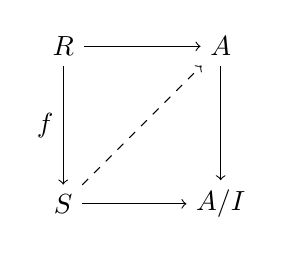
\begin{tikzpicture}
                \node (R) at (0, 1) {$R$};
                \node (S) at (0, -1) {$S$};
                \node (A) at (2, 1) {$A$};
                \node (AI) at (2, -1) {$A/I$};
                \draw[->] (R) -- node[left]{$f$} (S);
                \draw[->] (S) -- (AI);
                \draw[->] (R) -- (A);
                \draw[->] (A) -- (AI);
                \draw[->, dashed] (S) -- (A);
            \end{tikzpicture}
        \end{gather*}
        In other words, formally \'etale morphisms have the unique left lifting property with respect to infinitesimal thickenings. Saying that $f:R\rightarrow S$ is formally smooth (resp.~formally unramified) means that there exists at least (resp.~at most) one lift.
    }
    \begin{remark}[Topological rings]
        The previous definition can be generalized to \textit{topological rings} $R$ and $S$. In this case $A$ ranges over discrete algebras and all morphisms are taken to be continuous morphisms.
    \end{remark}

    \newdef{Completion\footnotemark}{\index{completion!of rings}\label{algebra:ring_completion}\index{formal!completion}\index{adic}
        \footnotetext{This form of ring completion is sometimes called the \textbf{formal completion} or \textbf{adic completion}.}
        Consider a commutative ring $R$ together with a proper ideal $I$. The completion $\widehat{R}$ of $R$ with respect to $I$ is the inverse limit $\varprojlim_{n\in\mathbb{N}}(R/I^n)$.
    }
    \begin{property}[Adic topology]\index{topology!adic}\index{Krull!topology}
        When the filtration ends in the trivial ideal, for example when $R$ is a Noetherian local ring, the completion $\widehat{R}$ is a topological ring (see \cref{chapter:topology}). The \textbf{Krull topology} or \textbf{$I$-adic topology} is the topology for which a basis of $0$ is given by the powers of $I$.
    \end{property}

    \begin{example}
        The completion of $R[x]$ with respect to $(x)$ is given by the ring of formal power series $R[[x]]$. In general, one can think of these completions as containing (formal) \textit{Taylor series expansions}.
    \end{example}

\subsection{Modules}

    \newdef{$R$-module}{\index{module!over a ring}\label{algebra:module}
        Let $(R,+,\cdot)$ be a ring. An Abelian group $(M,\oplus)$ is said to be a left $R$-module if there exists a left (monoid) action $\triangleright:(R,\cdot)\times M\rightarrow M$ that satisfies the following axioms:
        \begin{enumerate}
            \item\textbf{Left distributivity}: $r\triangleright(m\oplus n) = r\triangleright m\oplus r\triangleright n$ for all $r\in R$ and $m,n\in M$.
            \item\textbf{Right distributivity}: $(r+s)\triangleright m = r\triangleright m \oplus s\triangleright m$ for all $r,s\in R$ and $m\in M$.
        \end{enumerate}
        These conditions make sure that both the additive structure $(R,+)$ and the group structure $(M,\oplus)$ are compatible with the action of $(R,\cdot)$. Due to these compatibility conditions one can identify $\cdot\sim\triangleright$ and $+\sim\oplus$ without confusion.
    }
    \begin{remark}[\difficult{Categorical perspective}]
        The definition of a ring can be defined more concisely in categorical terms. Recall the definition of an algebra over a monad (\cref{cat:algebra_monad}). Modules over a monoid object $A$ are defined as algebras over the monad $A\otimes-$. A ring $R$ is a monoid object in the category $\mathbf{Ab}$ of Abelian groups. So a module $M$ over $R$ consists of a morphism $\alpha:R\otimes M\rightarrow M$ satisfying the algebra axioms. The distributivity laws come for free since $\alpha$ is a morphism in $\mathbf{Ab}$ and, hence, is bilinear (in both arguments).
    \end{remark}
    \newadef{$R$-module}{
        The above two formulations can be restated similar to that of group modules (\cref{group:module}). Consider the Abelian group $(M,\oplus)$. Its endomorphism set $\End(M,\oplus)$ can be given the structure of a ring where the addition is induced by that on $M$ and the multiplication is given by composition. A left $R$-module structure is then simply a ring morphism $R\rightarrow\End(M,\oplus)$.
    }

    \newdef{Morita equivalence}{\index{equivalence!Morita}\label{algebra:morita_equivalence}
        Two rings $R,S$ are said to be Morita equivalent if their categories of left modules (or, equivalently, right modules) are equivalent.
    }
    \begin{property}
        Two rings $R,S$ are Morita equivalent if and only if
        \begin{gather}
            S \cong eM_n(R)e
        \end{gather}
        for some $n\in\mathbb{N}$ and \textit{full idempotent} $e\in M_n(R)$.
    \end{property}

    \newdef{Bimodule}{\index{bi-!module}
        Let $R,S$ be two rings. An Abelian group $(M,\oplus)$ is an $R-S$-bimodule if
        \begin{enumerate}
            \item it is a left $R$-module,
            \item it is a right $S$-module, and
            \item the actions are compatible:
            \begin{gather}
                (r\triangleright m)\triangleleft s = r\triangleright(m\triangleleft s)
            \end{gather}
            for all $r\in R$, $s\in S$ and $m\in M$.
        \end{enumerate}
    }

    \newdef{Enveloping algebra}{\index{algebra!enveloping}\index{opposite!ring}\index{tensor product!of rings}\label{algebra:enveloping_algebra}
        Let $A$ be an \textit{algebra over a commutative ring} $R$ (see \cref{linalgebra:algebra_over_ring}). The enveloping algebra $A^e:=A\otimes\op{A}$ is defined as follows:
        \begin{gather}
            (a\otimes b)\cdot(a'\otimes b') := (a\cdot a')\otimes(b'\cdot b)
        \end{gather}
        for all $a,a',b,b'\in R$.\footnote{Note that this is simply a consequence of the definitions of the \textbf{opposite ring} ($a\cdot_{\text{op}}b:=b\cdot a$) and the \textit{tensor product of rings}.}
    }
    \newadef{Bimodule}{\index{bi-!module}
        Let $A$ be an algebra. An $A$-bimodule is a left $A^e$-module.
    }
    
    \newdef{Free module}{\index{free!module}\index{basis}
        An $R$-module $M$ that admits a \textbf{basis}, i.e.~there exists a set $\{x_i\}_{i\in I}$, where $I$ can be infinite, such that:
        \begin{enumerate}
            \item Every element $m\in M$ can be written as a linear combination $\sum_{j\in J_m}r_jx_j$, where $J_m\subseteq I$ is finite.
            \item The set $\{x_i\}_{i\in I}$ is linearly independent in the sense that
                \begin{gather}
                    \sum_{j\in J\subseteq I}r_jx_j=0\implies\forall j\in J:r_j=0.
                \end{gather}
        \end{enumerate}
    }
    \begin{example}[Dual numbers]\index{dual!numbers}
        Let $R$ be a ring. The $R$-algebra of dual numbers, often denoted by $R[\varepsilon]$, is defined as the free $R$-module with basis $\{1,\varepsilon\}$ subject to the relation $\varepsilon^2 = 0$.
    \end{example}

    \begin{property}[Division rings]\index{division!ring}\label{algebra:module_basis}
        For a general $R$-module, the existence of a basis is not guaranteed unless $R$ is a \textit{division ring}. (See \cref{linalgebra:hamel_basis} for more information.)
    \end{property}
    \begin{result}
        Since every field is in particular a division ring, the existence of a basis follows from the above property for $R$-modules.
    \end{result}

    \newdef{Projective module}{\index{projective!module}
        A module $P$ that can be expressed as
        \begin{gather}
            P\oplus M=F\,,
        \end{gather}
        where $M$ is a module and $F$ is a free module, i.e.~$P$ is projective if it is a direct sumand of a free module.
    }

    \begin{theorem}[Nakayama's lemma\footnotemark]\index{Nakayama lemma}\index{Krull--Azumaya}\label{algebra:nakayama}
        \footnotetext{Also called the \textbf{Krull--Azumaya lemma}.}
        Consider a commutative ring $R$. If $I\subset R$ is an ideal and $M$ a finitely generated $R$-module such that $IM=M$, there exists an element $r\in R$ with $r=1$ in $R/I$ such that $rM=0$.
    \end{theorem}
    The following corollary is also often called Nakayama's lemma:
    \begin{result}
        If $M$ is a finitely generated $R$-module and $J(R)M=M$, then $M=0$.
    \end{result}
    \begin{result}
        If $M$ is a finitely generated $R$-module and there exist elements $m_1,\ldots,m_k\in M$ whose image in $M/J(R)M$ generate this quotient, the elements generate $M$.
    \end{result}

\subsection{Semisimplicity}\index{semisimple!module}

    \newdef{Simple module}{\index{simple!module}
        A module over a ring that contains no nontrivial submodules. A module is said to be \textbf{semisimple} if it admits a decomposition as a direct sum of simple modules. A ring is said to be semisimple if it is semisimple as a module over itself.
    }
    \begin{property}[Jacobson radical]
        A ring is semisimple if and only if it is Artinian and if its Jacobson radical (\cref{algebra:jacobson_radical}) vanishes.
    \end{property}

    \begin{theorem}[Artin--Wedderburn]\index{Artin--Wedderburn}\label{algebra:artin_wedderburn}
        Every semisimple ring is isomorphic to a direct sum of matrix rings over division rings $D_i$ with multiplicity $n_i$. Furthermore, the integers $D_i$ and $n_i$ are unique (up to a permutation of the indices).
    \end{theorem}

\section{\difficult{Galois theory}}\index{Galois!theory}

\subsection{Polynomials}

    \newdef{Polynomial ring}{\index{poly-!nomial}\index{indeterminate}
        Let $R$ be a (commutative unital) ring and consider a set $X$. The polynomial ring on the \textbf{indeterminates} $X$ is defined as the free commutative $R$-algebra on $X$. Often, $X$ will be a finite set: $R[X]\equiv R[x_1,\ldots,x_n]$.
    }

    \begin{theorem}[Hilbert's basis theorem]\index{Hilbert!basis theorem}\label{algebra:hilbert_basis_theorem}
        If a ring is Noetherian (\cref{algebra:noetherian_ring}), any polynomial ring with finitely many indeterminates over it is also Noetherian.
    \end{theorem}

    \newdef{Irreducible polynomial}{\index{irreducible!polynomial}
        A polynomial that cannot be factorized as the product of two nonconstant polynomials. Over a field, a polynomial is irreducible if and only if the ideal it generates is maximal.
    }

    \newdef{Degree}{\index{degree!of polynomial}
        The degree of a polynomial $f$ is equal to the largest integer $d\in\mathbb{N}$ for which $f$ contains a monomial $x_1^{i_1}\cdots x_n^{i_n}$ such that $i_1+\cdots+i_n=d$. It is denoted by $\deg(f)$.
    }
    \newdef{Monic polynomial}{\index{monic}
        A polynomial for which the highest degree term has coefficient $1$.
    }

    \newdef{Split}{\index{split}\index{root}
        A polynomial $f\in R[x]$ is said to split (over $R$) if it can be factorized as a product of linear factors, i.e.~there exist elements $\lambda,r_1,\ldots r_n$ such that
        \begin{gather}
            f = \lambda(x-r_1)\cdots(x-r_n)\,,
        \end{gather}
        where $n=\deg(f)$. The numbers $r_i\in R$ are called the \textbf{roots} of the polynomial.
    }

    \begin{theorem}[Fundamental theorem of algebra]\index{fundamental theorem!of algebra}\label{alggeom:fundamental_theorem_of_algebra}
        Consider a $\mathbb{C}$-valued polynomial of degree $\geq 1$. It has at least one root in $\mathbb{C}$.
    \end{theorem}
    \begin{result}
        If $f\in \mathbb{C}[x]$ is a monic polynomial with $\deg(f)\geq1$, it can be factorized as follows:
        \begin{gather*}
            f(x) = \prod_{i=1}^k(x-a_i)^{n_i},
        \end{gather*}
        where $a_1,\ldots, a_k\in\mathbb{C}$ and $n_1,\ldots,n_k\in\mathbb{N}$.
    \end{result}

    \begin{formula}[Vieta]\index{Vieta}
        Consider a polynomial of degree $n$. By the fundamental theorem of algebra, this polynomial has $n$ complex roots. Vieta's formulas relate the coefficients of the polynomial to its roots $r_i$:
        \begin{gather}
            \sum_{1\leq i_1\leq\ldots\leq i_k\leq n}\ \prod_{j=1}^kr_{i_j} = (-1)^k\frac{a_{n-k}}{a_n}\,,
        \end{gather}
        where $k\leq n$. For $k=1$ and $k=n$, this gives the well-known sum and product formulas:
        \begin{align}
            r_1+r_2+\cdots+r_n &= -\frac{a_{n-1}}{a_n}\,,\\
            r_1r_2\cdots r_n &= (-1)^n\frac{a_0}{a_n}\,.
        \end{align}
    \end{formula}
    \begin{example}
        For quadratic polynomials
        \begin{gather}
            f(x) = ax^2+bx+c\,,
        \end{gather}
        one recovers the following well-known formulas:
        \begin{align}
            r_1+r_2 &= -\frac{b}{a},\\
            r_1r_2 &= \frac{c}{a}\,.
        \end{align}
    \end{example}

\subsection{Field extensions}

    \newdef{Field extension}{\index{field!extension}\label{algebra:field_extension}
        Let $K$ be a field. A field extension of $K$ is a field $L$ such that $K\subseteq L$ and such that the operations of $K$ are the restrictions of those in $L$.
    }
    \begin{notation}
        A field extension $L$ of $K$ is often denoted by $L/K$.
    \end{notation}

    \begin{notation}[Generation]\index{simple!extension}
        Consider a field extension $L/K$ together with a subset $X\subseteq L$. The smallest field extension of $K$ that contains $X$ is denoted by $K(X)$. $L$ is said to be \textbf{simple} if $L=K(a)$ for some $a\in L$.
    \end{notation}

    \newdef{Degree}{\index{degree!of field extension}\index{extension!finite}
        If $L/K$ is a field extension, $L$ can be given the structure of a $K$-\textit{vector space} (see \cref{linalgebra:vector_space}). The dimension of this vector space is called the degree of the extension $K$. It is often denoted by $[L:K]$. If the degree is finite, the extension is also said to be \textbf{finite}.
    }

    The following property is very similar to the tower rule for finite groups (\cref{group:tower_rule_groups}).
    \begin{property}[Tower property]\index{tower law}
        Consider two field extensions $M/L$ and $L/K$.
        \begin{gather}
            [M:K]=[M:L][L:K]
        \end{gather}
    \end{property}
    \sremark{Galois theory will show that this is no mere coincidence.}

    \newdef{Number field}{\index{number!field}\label{algebra:number_field}
        A finite extension of the rational numbers $\mathbb{Q}$.
    }

\subsection{Algebraicity}\label{section:algebraic_numbers}

    \newdef{Algebraic element}{\index{transcendental}\index{algebraic}\label{algebra:algebraic_element}
        Consider a field extension $L/K$. An element $x\in L$ for which there exists a nontrivial polynomial $p\in K[x]$ such that $p(x)=0$, is said to be algebraic, otherwise it is said to be \textbf{transcendental}.
    }

    \newdef{Algebraic dependence}{
        Consider a commutative ring $R$ and a subring $S\subset R$. An element $r\in R$ is said to be algebraically dependent on $S$ if it is the root of a polynomial in $S[x]$. If $r$ is the root of a monic polynomial in $S[x]$, it is said to be \textbf{integrally dependent} on $S$.
    }
    \begin{remark}
        Since every nonzero element in a field is invertible, one can always turn a general polynomial into a monic polynomial. Hence, over a field, the concepts of algebraic and integral dependence coincide.
    \end{remark}

    \newdef{Algebraic integer}{\index{integer!algebraic}\label{algebra:algebraic_integer}
        Let $K$ be a number field. An algebraic integer of $K$ is an element satisfying a polynomial with integer coefficients.
    }

    \newdef{Algebraic extension}{\index{extension!algebraic}
        An extension $L/K$ such that every element of $L$ is algebraic over $K$.
    }

    \begin{property}
        Every finite extension is algebraic.
    \end{property}

    \newdef{Algebraic closure}{\index{algebraic!closure}\label{algebra:algebraic_closure}
        A field is said to be \textbf{algebraically closed} if every polynomial over it has a root. This implies that every polynomial splits. An algebraic closure of a field $K$ is an algebraic extension $\overline{K}/K$ such that $\overline{K}$ is algebraically closed.
    }
    \newdef{Splitting field}{\index{splitting field}\label{algebra:splitting_field}
        Consider a field $K$ and a polynomial $f\in K[x]$. The smallest field extension of $K$ over which $f$ splits is called the splitting field of $f$.
    }
    \begin{property}
        A splitting field of a polynomial of degree $n$ has degree at most $n!$.
    \end{property}
    \begin{example}
        \Cref{alggeom:fundamental_theorem_of_algebra} implies that $\mathbb{C}$ is an algebraic closure of $\mathbb{R}$. In fact, it is also the splitting field over $\mathbb{R}$.
    \end{example}

    \newdef{Minimal polynomial}{\index{minimal!polynomial}\index{evaluation}\label{algebra:minimal_polynomial}
        Consider a field extension $L/K$ with an element $a\in L$ that is algebraic over $K$. The monic polynomial $f^a\in K[x]$ of lowest order such that $f^a(a)=0$ is called the minimal polynomial of $a$. This polynomial is obtained as the generator\footnote{Polynomial rings in one variable are PIDs, so the kernel ideal admits a generator.} of the kernel ideal of the \textbf{evaluation morphism}
        \begin{gather}
            K[x]\rightarrow L:f\mapsto f(a)\,.
        \end{gather}
    }
    \begin{property}\label{algebra:minimal_polynomial_divisor}
        Let $f^a$ be the minimal polynomial of an algebraic element $a\in L$. If $f(a)=0$ for some polynomial $f\in K[x]$, the minimal polynomial $f^a$ divides $f$.
    \end{property}
    \begin{result}
        The minimal polynomial of an algebraic element is irreducible.
    \end{result}

    \begin{property}
        Consider two fields $K,L$ together with an element $a\in L$. The `polynomial ring' $K[a]$, the image of the evaluation morphism, coincides with $K(a)$ if and only if $a$ is algebraic over $K$.
    \end{property}

    \newdef{Separable element}{\index{separable}
        An element $a\in\overline{K}$ of an algebraic closure $\overline{K}/K$ is said to be separable (over $K$) if the minimal polynomial $f^\alpha\in K[x]$ is separable, i.e.~has no multiple zeros. A subextension $L\subset\overline{K}$ is said to be separable if every element of $L$ is separable over $K$.
    }
    \newdef{Separable closure}{\index{separable!closure}\label{algebra:separable_closure}
        Let $K$ be a field with algebraic closure $\overline{K}$. The separable closure $K_S$ is defined as follows:
        \begin{gather}
            K_S := \{x\in\overline{K}\mid x\text{ is separable over }K\}\,.
        \end{gather}
    }
    \begin{example}[Separable splitting field]
        The splitting field of a separable polynomial is separable.
    \end{example}

    \newdef{Perfect field}{\index{perfect!field}
        A field $K$ satisfying any of the following equivalent statements:
        \begin{enumerate}
            \item Every irreducible polynomial over $K$ is separable.
            \item Every algebraic extension of $K$ is separable.
            \item Every finite extension of $K$ is separable.
            \item The separable closure $K_S$ is algebraically closed.
        \end{enumerate}
    }
    \begin{example}
        All finite fields and fields of characteristic zero are perfect.
    \end{example}
    \begin{result}
        For a perfect field, the algebraic closure and separable closure coincide.
    \end{result}

    \newdef{Normal extension}{\index{extension!normal}
        A field extension $L/K$ with $L\subseteq\overline{K}$ is said to be \textbf{normal} if every irreducible polynomial in $K[x]$ that has a root in $L$ splits over $L$.
    }
    \begin{property}
        A field extension is normal if and only if it is the splitting field for some set of polynomials. Moreover, it is finite normal if and only if it is the splitting field of a single polynomial.
    \end{property}

    \newdef{Normal closure}{\index{normal!closure}
        Consider a field extension $L/K$. The normal closure of $L$ is the smallest normal extension of $L$ over $K$.
    }

\subsection{Galois extensions}

    \newdef{Galois extension}{\index{Galois!extension}\index{Krull!topology}\index{group!profinite}
        An algebraic field extension $L/K$ such that there exists a subgroup $G\subseteq\Aut(L)$ satisfying
        \begin{gather}
            K\cong L^G\,,
        \end{gather}
        where $L^G$ denotes the set of $G$-invariants of $L$. This group, often denoted by $\mathrm{Gal}(L/K)$, is called the \textbf{Galois group} of the extension. If $L$ is the splitting field of a polynomial $f\in K[x]$, the Galois group is sometimes denoted by $\mathrm{Gal}(f)$.

        When $L/K$ is finite, the Galois group is a finite group and, hence, can simply be endowed with the discrete topology. However, when the extension is not finite, one should endow the group with a topology. The \textbf{Krull topology} is defined as the \textit{profinite topology} (see \cref{topology:profinite_group}) with respect to all finite subgroups of $\mathrm{Gal}(L/K)$.\footnote{One can show that every \textit{profinite group} arises as the Galois group for some field extension.}
    }

    \begin{property}
        Consider a field extension $L/K$. The following statements are equivalent:
        \begin{itemize}
            \item $L$ is a Galois extension.
            \item $L$ is algebraic, normal and separable over $K$.
        \end{itemize}
    \end{property}
    \begin{property}
        A finite extension $L/K$ is Galois if and only if $|\mathrm{Gal}(L/K)|=[L:K]$.
    \end{property}

    \begin{theorem}[Fundamental theorem of Galois theory]\index{fundamental theorem!of Galois theory}
        Consider a Galois extension $L/K$. The intermediate field extensions $K'/K$ are in bijection with the closed subgroups of $\mathrm{Gal}(L/K)$.
    \end{theorem}
    \begin{property}
        Consider a subgroup $H\subset\mathrm{Gal}(L/K)$. The correspondence in the fundamental theorem has the following properties:
        \begin{itemize}
            \item $L/L^H$ is Galois.
            \item If $H$ is open, $L^H/K$ is finite.
            \item If $H$ is normal, $L^H/K$ is Galois with $\mathrm{Gal}\left(L^H/K\right)\cong\mathrm{Gal}(L/K)/H$.
        \end{itemize}
    \end{property}

\subsection{Radicals}

    \newdef{Radical extension}{\index{extension!radical}\index{radical|seealso{extension}}
        A simple radical extension $L/K$ is a simple extension $L=K(a)$ such that $a^n=b$ for some $b\in K$ and $n\in\mathbb{N}_0$. A radical extension or radical series is a finite sequence of simple radical extensions.
    }

    \begin{property}
        If $L/K$ is radical and $K'$ is an intermediate field extension, $\Aut(K'/K)$ is solvable.
    \end{property}

    \begin{theorem}[Galois]
        A polynomial $f\in K[x]$, where $\mathrm{char}(K)$ does not divide $\deg(f)$, can be solved by radicals if and only if its Galois group $\mathrm{Gal}(f)$ is solvable (\cref{group:solvable}).
    \end{theorem}

    \todo{COMPLETE}

\subsection{Nullstellensatz}\index{Nullstellensatz}

    For the geometric incarnation, see \cref{chapter:alggeom}.

    \begin{theorem}[Weak Nullstellensatz]
        Let $K$ be an algebraically closed field and consider the polynomial ring $R=K[x_1,\ldots,x_n]$. An ideal $I\subset R$ is maximal if and only if it is of the form \[(x_1-a_1,\ldots,x_n-a_n)\] with $a_i\in K$ for all $i\leq n$.
    \end{theorem}
    \begin{result}
        There exists a bijection between $K^n$ and the set of maximal ideals of $K[x_1,\ldots,x_n]$.
    \end{result}
    \begin{result}
        Consider a collection of polynomials $\{f_i\}_{i\in I}\subset K[x_1,\ldots,x_n]$. If these polynomials do not have a common root, the ideal they generate is the unit ideal.
    \end{result}

    \todo{COMPLETE}